\documentclass[20pt]{extarticle}
% \usepackage[paperwidth=48in, paperheight=36in]{geometry}
\usepackage{better_poster}


% ---- fill in from here

% authors
\title{}
\author{}

% type of poster: [exp]erimental results, [methods], [theory]
% Disclaimer: the original classification had "study" and "intervention" as separate categories. I group them under experimental results.
\newcommand\postertype{exp} % [exp],[methods],[theory]

\begin{document}
\fontsize{38pt}{28pt}\selectfont


\newfinding{
\Huge \textbf{PyLinguist: A Python code to Hindi code translator}\\
\LARGE \textbf{Authors:} \textit{Ankit Kumar, Antara Tewary, Homa Haghighi}
}
% \vspace{-15pt}

% % the main text of your poster goes here
\vspace{-10pt}
\makemain{
    \vspace{-1.5 cm}
\begin{tcolorbox}[title= \centering {Introduction}]
    \begin{itemize}
        \item \textbf{Problem:} 
              Translation of Python code to Hindi is challenging due to the lack of a comprehensive translation system.
        
        \item \textbf{Objective:} 
              Develop a translation system that accurately converts English Python code to Hindi.
        
        \item \textbf{Approach:} 
              A hybrid translation system combining keyword preservation and GPT-4o-mini.
    \end{itemize}
    
\end{tcolorbox}
\vspace{1cm}

\begin{tcolorbox}[title= \centering {Motivation}]
    \begin{itemize}
        \item \textbf{Accessibility:} 
              Facilitate learning and understanding of Python programming for Hindi speakers.
        
        \item \textbf{Inclusivity:} 
              Enable Hindi speakers to access Python resources and contribute to the programming community.
        
        \item \textbf{Efficiency:} 
              Enhance productivity by providing a comprehensive translation system for Python code.
    \end{itemize}
\end{tcolorbox}
\vspace{1cm}

\begin{tcolorbox}[title=\centering {System Architecture}]
    \begin{itemize}
        \item \textbf{Frontend:} Streamlit-based web interface with dual code editors.
        
        \item \textbf{Translation Engine:} Hybrid system combining keyword preservation and GPT-4o-mini.
            \begin{itemize}
                \item Dictionary based keyword translation
                \item Deep translation using google translate to translate non-keyword elements
                \item Syntax preservation mechanism
            \end{itemize}
        
        \item \textbf{Data Management:} 
              checkpointing and logging for translation data.
    \end{itemize}
\end{tcolorbox}
}
% If you have extra figures or data to show
\makeextracolumn{
\vspace{-0.1cm}
\begin{tcolorbox}[title= \centering Technical Implementation]
    \begin{itemize}
        \item \textbf{Stage 1 - Base Translation:} 
              Implementation of a hybrid translation system combining keyword preservation and Google Translate:
              \begin{itemize}
                  \item Keyword dictionary maintains Python-specific term translations
                  \item Parser identifies code components (variables, comments, strings)
                  \item Google Translate handles non-keyword elements
              \end{itemize}
        
        \item \textbf{Stage 2 - GPT Enhancement:} 
              Example-based translation using GPT-4o-mini:
              \begin{itemize}
                  \item Utilizes successful translations from Stage 1 as examples
                  \item Performs partial translation using keyword dictionary
                  \item GPT model completes translation based on examples
              \end{itemize}
        
        \item \textbf{Stage 3 - Quality Assessment:} 
              Comprehensive evaluation framework:
              \begin{itemize}
                  \item Back-translation verification
                  \item Syntax validation 
                  \item BLEU score evaluation 
                  \item Semantic preservation testing
              \end{itemize}
    \end{itemize}
\end{tcolorbox}
\vspace{1cm}
\begin{tcolorbox}[title= \centering Challenges]
    \begin{itemize}
        \item \textbf{Syntax Preservation:} 
              Maintaining code structure and functionality during translation.
        
        \item \textbf{Keyword Translation:} 
              Accurate translation of Python-specific terms to Hindi.
        
        \item \textbf{Evaluation:} 
              Developing a robust framework for translation quality assessment.
    \end{itemize}
\end{tcolorbox}

}
\thirdcolumn{
\vspace{-0.1cm}
\begin{tcolorbox}[title= \centering {Evaluation Framework}]
    \begin{itemize}
        \item \textbf{Back-translation Verification:} 
              Translation of Hindi code back to English for comparison.
        
        \item \textbf{Syntax Validation:} 
              Verification of code structure and functionality.
        
        \item \textbf{BLEU Score Evaluation:} 
              Comparison of translated code with reference translations.
        
        \item \textbf{Semantic Preservation Testing:} 
              Evaluation of code functionality and logic.
    \end{itemize}
    
\end{tcolorbox}
\vspace{1cm}

\begin{tcolorbox}[title= \centering Results]
    \begin{itemize}
        \item Successful translation of Python code for Hindi languages. 
        \item Preservation of code functionality and structure.
        \item High accuracy in translation of Python keywords.
        \item Robust evaluation framework for translation quality assessment.
        \item potential for further improvement and expansion.
            %   \begin{itemize}
            %       \item Back-translation verification
            %       \item Syntax validation 
            %       \item BLEU score evaluation 
            %       \item Semantic preservation testing
            %   \end{itemize}
    \end{itemize}
\end{tcolorbox}
\vspace{1cm}
\begin{tcolorbox}[title= \centering Conclusion]
    \begin{itemize}
        \item \textbf{PyLinguist:} 
              A comprehensive translation system for English Python code to Hindi.
        
        \item \textbf{Future Work:} 
              \begin{itemize}
                  \item Expand translation system to other languages
                  \item Improve translation accuracy
                  \item Develop a user-friendly interface
              \end{itemize}
    \end{itemize}
\end{tcolorbox}
}


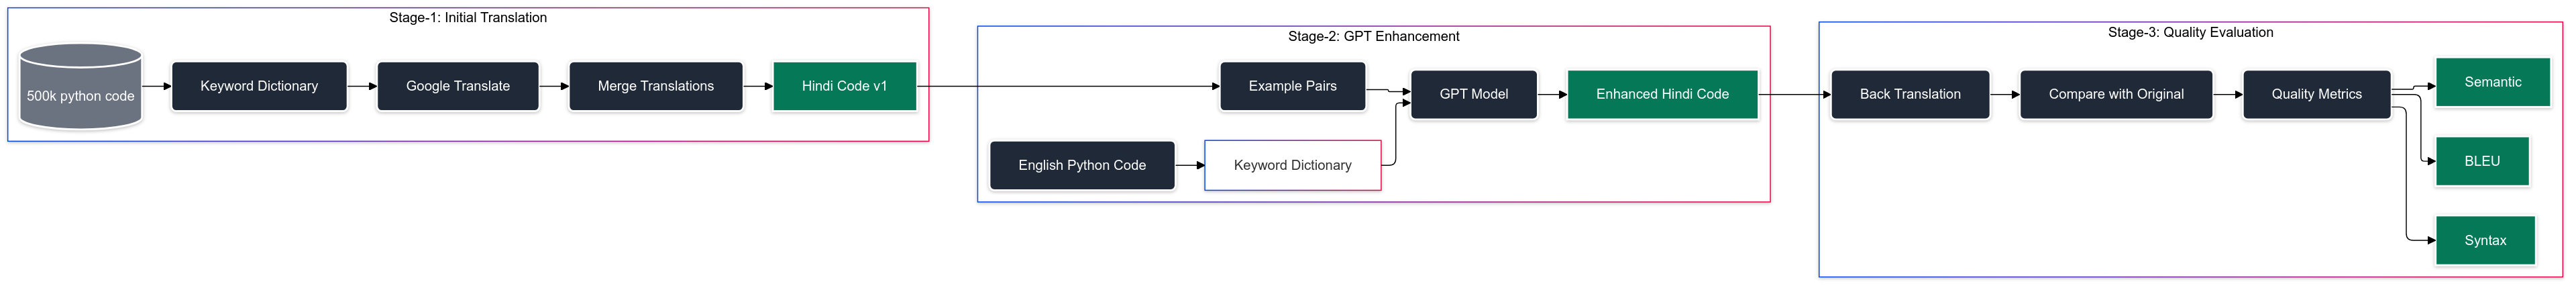
\includegraphics[width=\textwidth]{images/final-flow-1.png}

    

% footer
% generate qr code from https://www.qr-code-generator.com/ and replace qr_code.png
% default: barcode on the left
% \makefooter{images/GMUNLP.pdf}{images/qr-code.pdf}

% replace with this like for barcode on the right
\makealtfooter{images/qrcode_with_border.png}
 
\end{document}